% Setup
\documentclass[16pt]{article}
\usepackage{graphicx}
\usepackage{fullpage}

\usepackage{caption}
\usepackage{subcaption}

\setlength{\textwidth}{9in}
\setlength{\evensidemargin}{-0.8in}
\setlength{\oddsidemargin}{-0.8in}

% Font
\usepackage[scaled]{helvet}			       % Helvetica
\renewcommand*\familydefault{\sfdefault}        % Only if the base font of the document is to be sans serif
\usepackage[T1]{fontenc}

% Variables for our figure
\newcommand{\figPath}[1]{../../../data/parametricConditions2/c32_pnt_rot0_shad4_blk40_cen40_vs_shd_rot0_shad4_blk40_cen40_t1/#1}
\newcommand{\panelWidth}{0.40\textwidth}
\newcommand{\figWidth}{0.6\textwidth}
\newcommand{\panelFont}[1]{{\fontsize{16pt}{14pt}\selectfont #1}}
\newcommand{\fignameFont}[1]{{\fontsize{18pt}{14pt}\selectfont #1}}

\begin{document}
\pagenumbering{gobble}

\begin{figure}
        \centering
        
        	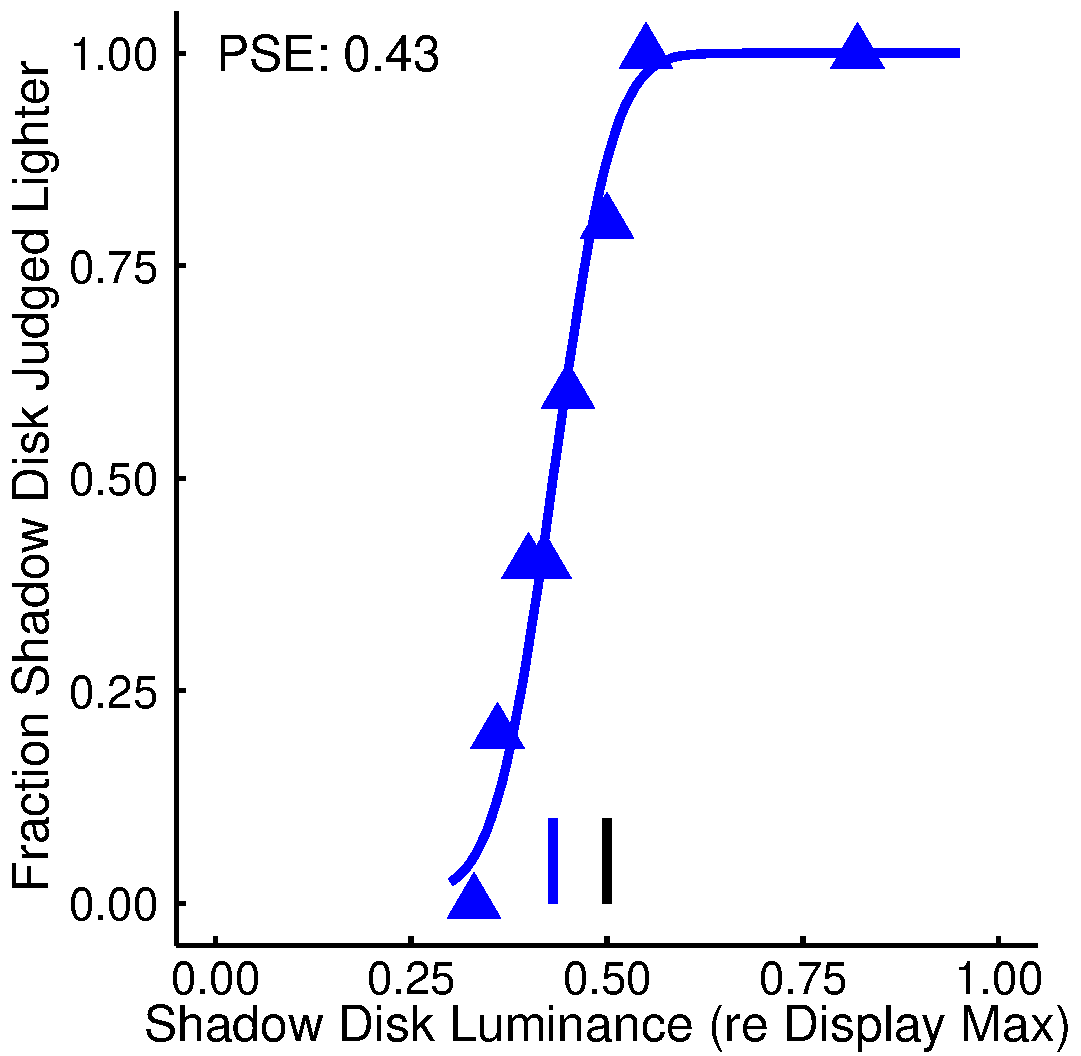
\includegraphics[width=\figWidth]{\figPath{aqr/aqr-c32_pnt_rot0_shad4_blk40_cen40_vs_shd_rot0_shad4_blk40_cen40_t1-2_exampleOne.pdf}}
            
\end{figure}

% Figure number
\vspace{0.6in}
\centering
\fignameFont{Psychophysics Figure 1}
        
\end{document}
